\subsection{Reporte de exploración de los datos}

\subsubsection*{Distribución del BCS y su relación con MAE y accuracy}

\begin{figure}[H]
  \centering
  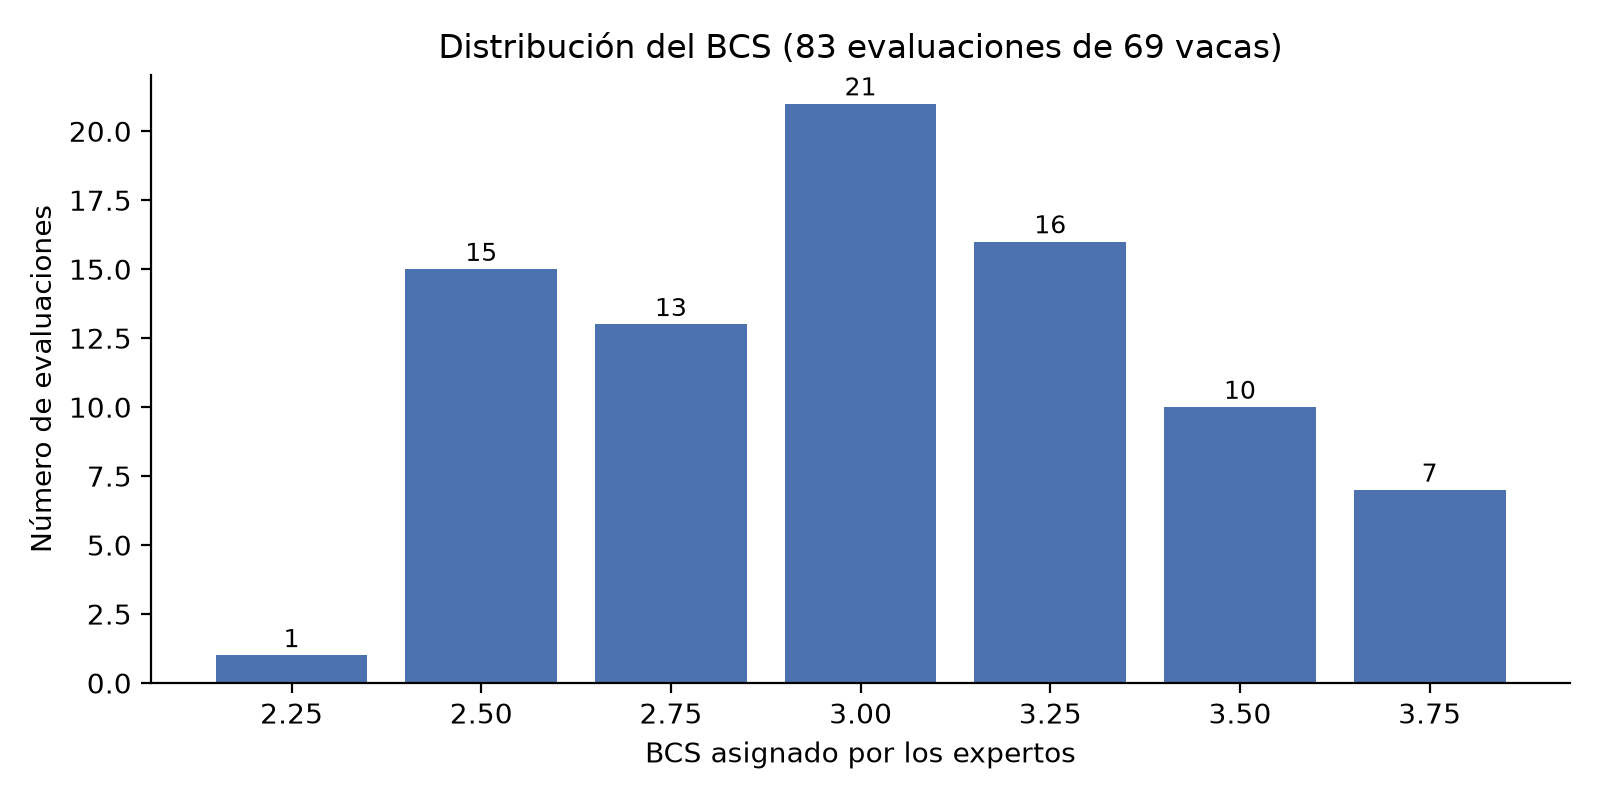
\includegraphics[width=0.85\textwidth]{figures/distribucion_bcs.png}
  \caption{Distribución del BCS asignado por los expertos.}
  \label{fig:distribucion-bcs}
\end{figure}

\begin{table}[H]
  \centering
  \caption{Evaluaciones por clase de BCS.}
  \label{tab:distribucion-bcs}
  \begin{tabular}{lrr}
    \toprule
    BCS & Evaluaciones & Porcentaje \\
    \midrule
    2.25 & 1 & 1.2\% \\
    2.50 & 15 & 18.1\% \\
    2.75 & 13 & 15.7\% \\
    3.00 & 21 & 25.3\% \\
    3.25 & 16 & 19.3\% \\
    3.50 & 10 & 12.0\% \\
    3.75 & 7 & 8.4\% \\
    \bottomrule
  \end{tabular}
\end{table}

La clase más frecuente es 3.0, con 21 evaluaciones (25.3\%). Las clases de los extremos tienen pocas evaluaciones: 2.25 tiene 1 y 3.75 tiene 7. No hay evaluaciones menores a 2.25 ni mayores a 3.75, así que el modelo no verá vacas fuera de ese rango.

Esta distribución es importante para las dos métricas que definimos. Con pocas vacas por clase, la accuracy puede cambiar mucho con un solo error, y el MAE depende de qué tan lejos quedan las clases extremas del centro de la distribución.

De las 14 vacas con dos evaluaciones, la diferencia entre ellas es de 0.125 en promedio y de 0.25 como máximo, y en 7 vacas las dos evaluaciones son iguales. Esto sirve como referencia de cuánto varía el BCS cuando lo asigna una persona experta.

\subsubsection*{Cruce entre fotos, conjunto de datos y BCS de expertos}

Cruzamos las 69 vacas con BCS con el conjunto de datos de VMS 3 (24 vacas) y con los datos de ordeño (34 vacas).

\begin{table}[H]
  \centering
  \caption{Cruce de las fuentes de datos.}
  \label{tab:cruce}
  \begin{tabular}{lr}
    \toprule
    Cruce & Vacas \\
    \midrule
    Con BCS de los expertos & 69 \\
    Con BCS y en VMS 3 & 13 \\
    Con BCS y con datos de ordeño & 12 \\
    En las tres fuentes & 2 (2082 y 8709) \\
    En VMS 3 sin BCS de los expertos & 11 \\
    \bottomrule
  \end{tabular}
\end{table}

Las 13 vacas con BCS que están en VMS 3 son 1532, 1543, 1547, 1564, 1567, 2082, 2142, 6137, 8709, 8744, 8799, 91549 y 91561.

De esas 13 vacas, 12 tienen valor en ``Evento BCS''. Comparado con el BCS de los expertos, ``Evento BCS'' es mayor en 9 vacas, igual en 2 y menor en 1, y en promedio queda 0.43 puntos arriba. Como desconocemos qué mide esta columna, no se debe usar como si fuera el BCS de los expertos.

\subsubsection*{Relación con los datos de ordeño}

De las 34 vacas con datos de ordeño, 12 tienen BCS de los expertos: 1204, 1221, 1554, 1624, 1634, 2076, 2082, 6178, 8709, 8729, 8758 y 8775. De ellas, solo la 2082 y la 8709 están también en VMS 3.

Los datos de ordeño siguen siendo contexto, porque cubren menos de la quinta parte de las vacas con BCS y sus fechas son de más de un año antes de las fotos. Por eso consideramos que su relación con el BCS no es significativa y no los usaremos como variables del modelo.

\subsubsection*{Exploración de los datos de ordeño (contexto)}

La tabla~\ref{tab:ordeno-resumen} resume las principales variables. La columna ``Global'' pondera a cada vaca por su número de ordeños. Las demás columnas comparan a las vacas entre sí y usan solo las 31 vacas con al menos 30 ordeños, porque tres vacas (1497, 8771 y 8775) tienen muy pocos datos para que sus promedios sean comparables.

\begin{table}[H]
  \centering
  \small
  \caption{Resumen de las variables de ordeño.}
  \label{tab:ordeno-resumen}
  \begin{tabularx}{\textwidth}{>{\raggedright\arraybackslash}Xrrrrr}
    \toprule
    Variable & Global & Media & Mediana & Mínimo & Máximo \\
    \midrule
    Ordeños por vaca & 7016 (34 vacas) & 206.4 & 244.5 & 1 & 419 \\
    Producción por ordeño (kg) & 13.72 & 13.53 & 13.86 & 7.66 & 18.85 \\
    Producción diaria (kg) & 31.12 & 30.45 & 28.13 & 13.15 & 55.50 \\
    Ordeños por día & 2.27 & 2.21 & 2.14 & 1.45 & 3.17 \\
    Duración media (min) & 8.48 & 8.24 & 7.83 & 5.36 & 13.51 \\
    Ordeños con patada (\%) & 18.5 & 18.2 & 15.2 & 0.7 & 62.2 \\
    Ordeños incompletos (\%) & 14.5 & 13.8 & 8.5 & 0.0 & 57.9 \\
    Ordeños con pezones no encontrados (\%) & 17.7 & 16.3 & 5.1 & 0.0 & 83.3 \\
    \bottomrule
  \end{tabularx}
\end{table}

La media, la mediana, el mínimo y el máximo son entre vacas. La producción diaria es la producción total entre los días en que la vaca tuvo al menos un ordeño.

\begin{figure}[H]
  \centering
  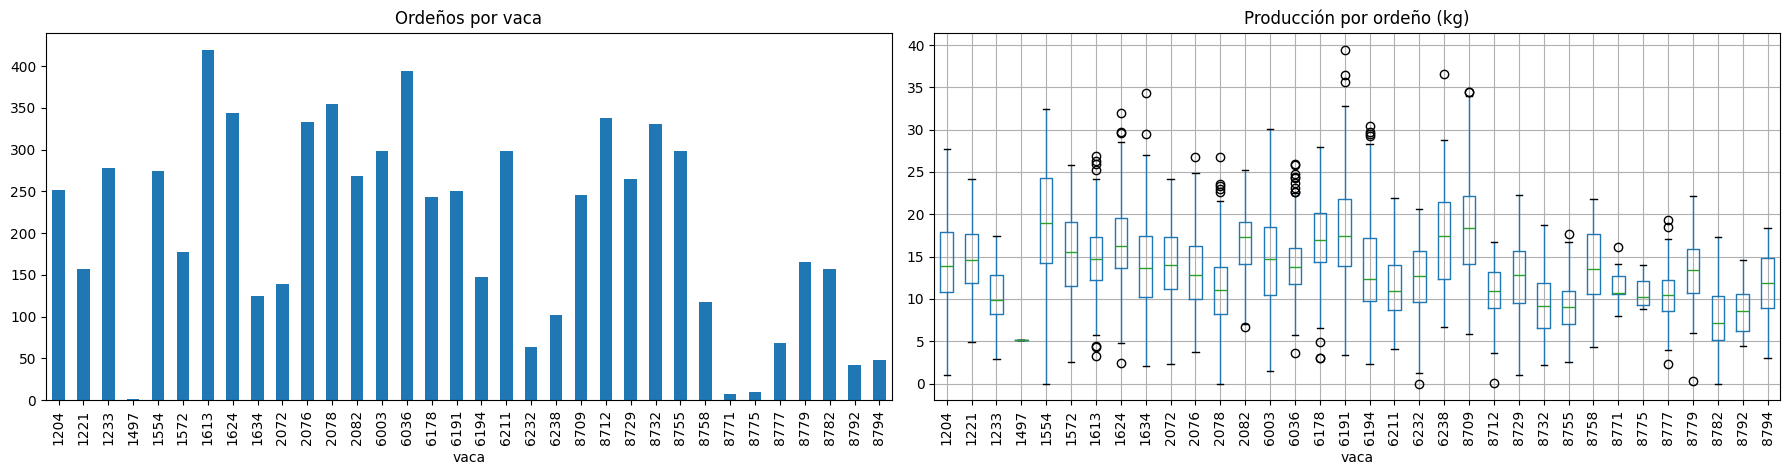
\includegraphics[width=\textwidth]{figures/ordenos_produccion_por_vaca.png}
  \caption{Ordeños por vaca y producción por ordeño (kg) de cada vaca.}
  \label{fig:ordenos}
\end{figure}

\begin{itemize}
  \item \textbf{Producción:} el promedio global fue de 13.7 kg por ordeño y la mediana entre vacas de 13.9 kg. La vaca con mayor promedio fue la 1554, con 18.9 kg por ordeño, y la de menor promedio entre las comparables fue la 8782, con 7.7 kg. Cinco vacas (1554, 2078, 6232, 8782 y 8712) tuvieron ordeños con 0 kg o 0.08 kg.
  \item \textbf{Frecuencia y duración:} las vacas se ordeñan en promedio 2.27 veces al día. El intervalo mediano entre ordeños va de 7.0 horas (vaca 6003) a 14.8 horas (vacas 8792 y 8794). Un ordeño dura en promedio 8.5 minutos. La vaca más rápida promedió 5.4 minutos (8712) y la más lenta 13.5 minutos (8755).
  \item \textbf{Incidentes:} se concentran en muy pocas vacas. Las vacas 8755, 8732 y 6003 tienen entre 45\% y 83\% de sus ordeños con pezones no encontrados o incompletos, y la 2076 tiene patada en el 62.2\% de sus ordeños.
  \item \textbf{Conductividad:} la media por cuarto va de 3.82 mS/cm (TD) a 4.74 mS/cm (DD). Los ordeños con más de 6.0 mS/cm son pocos en todos los cuartos (entre 0.9\% y 2.8\%), pero se concentran en algunas vacas, como la 6178 en el cuarto DI (23.1\%).
  \item \textbf{Sangre:} solo 431 lecturas de cuarto tienen sangre mayor a 0 ppm, menos del 2\% del total.
  \item \textbf{Estado AMD:} el estado AMD de la ubre vale 1 en 1050 de los 7016 ordeños (15.0\%). Por ahora solo consideramos su frecuencia, porque su significado debe confirmarse con el CAETEC.
  \item \textbf{Robots:} sobre las 7249 filas, VMS 3 registró 4276 (59.0\%), VMS 2 registró 1674 (23.1\%) y VMS 1 registró 1299 (17.9\%).
  \item \textbf{Cobertura temporal:} 14 vacas tienen datos en prácticamente todo el rango de 140 días, 12 empiezan después del 01/03/2025 y 6 tienen ausencias prolongadas de entre 54 y 104 días. El socio formador explicó que esos huecos pueden corresponder al periodo seco de la vaca.
\end{itemize}

\textbf{Destino de la leche.} La tabla~\ref{tab:destino} muestra a dónde fue la leche de los 7016 ordeños. Desviar la leche significa que su destino no es el tanque, donde se mezcla la leche de todas las vacas. Hubo 244 ordeños con leche desviada, de los cuales 152 fueron al drenaje y 92 a Divert 3. Según el socio formador, si la leche tiene sangre o microbios se desecha.

\begin{table}[H]
  \centering
  \caption{Destino de la leche.}
  \label{tab:destino}
  \begin{tabular}{lrr}
    \toprule
    Destino & Ordeños & Porcentaje \\
    \midrule
    Tanque & 6772 & 96.5\% \\
    Drenaje & 152 & 2.2\% \\
    Divert 3 & 92 & 1.3\% \\
    Total de ordeños & 7016 & 100\% \\
    \bottomrule
  \end{tabular}
\end{table}

Trece vacas enviaron menos del 95\% de su leche al tanque. El caso más destacable es la 6003, que solo envió el 71.5\% (213 de 298 ordeños). La columna ``Razón de la desviación'' tiene un único valor en todo el conjunto, así que no explica los 244 ordeños desviados.
